\section{「\dots 甘いものって\dots 好き？」}
\rightline{（文責：葛城リーリヤ）}

\subsection{ティーパーティー新歓の紹介}
　5月にティーパーティー新歓があります。おいしいスイーツとおいしい飲み物を楽しみながら、まったりと親睦を深める新歓です。新入寮生の皆さん、ぜひご参加ください。スイーツは有志の製作者が各々の知恵を絞り、腕を振るったもので多種多様です。（ちなみに、去年は以下のものが提供されました。ザッハトルテ、スコーン、白玉、モンブラン、チョコチップクッキー、マドレーヌ、フルーツ飴、サーターアンダギー、バスク風チーズケーキ、クレープ、チョコレートフォンデュ）余談ですが、しょっぱい系を出してくれるありがたい人が例年現れます。去年はクレープがおかず系のもありました。

\subsection{お菓子作りの魅力}
　この生地ではティーパーティー新歓でお菓子を出している一寮生（私）がお菓子作りの魅力をアピールするとともに、お菓子作りが持つ可能性と熊野寮でのその実現について語ります。お菓子以外の料理が好きな人、料理に挑戦してみたい人も共通する部分があると思うので読んでもらえたら嬉しいです。
　お菓子を作ったことはありますか？あれを作りたいと思ってレシピを調べるとバニラエッセンスやベーキングパウダーといった持ってない材料がある。いざ作ろうと思うと分量を細かく量らないといけなくてめんどくさい。どのくらい混ぜたらいいのかわからない。そもそも道具がない。頑張って作ったのに結局おいしくなかった。こんな経験でお菓子作りを諦めてしまう人が多いのではないか、と推測します。しかし、お菓子作りは、もっと楽しく、簡単で、おいしいものです。
　お菓子作りの多くはだれにでもできるものです。もし突然、魚を捌いてと頼まれてできる人は少ないと思いますが、これを混ぜてと頼まれたら大体の人は何とかなります。そして、お菓子作りの工程には多くの場合で意味があります。例えばバターをクリーム状になるまで混ぜることで、溶かさずにほかの材料と混ぜ、焼く際に溶けることでサクサクになります、卵の白身を分けて泡立ててメレンゲを作り、混ぜることで出来上がりがふわふわになります。自分が一つ一つの工程を積み上げることで、一つ一つの材料が生地へと変化していく様子を楽しむことができます。私もこの作業すること自体が好きですし、キャラクターの葛城リーリヤもストレス発散でお菓子を作りすぎてしまうみたいです。その一方で、液体の生地をオーブンに入れると、次にオーブンを開けた時にはおいしいお菓子が出来上がっているという魔法のような面白さもあります。自分でお菓子を作ることで費用も抑えられます。お菓子の材料の小麦粉、牛乳、卵、砂糖あたりは比較的安いですし、それらを使ったレシピもたくさんあります。何より、自分で作るということは焼きたてを好きなだけ食べられるということです。自分が作ったことも相まって、幸せな気持ちになります。

\subsection{熊野寮におけるお菓子作り環境}
　お菓子作りにハードルがあるのは事実かもしれません。しかし、これらのハードルの数々は熊野寮ではぐんと低くなります。熊野寮にはお菓子づくりに向いているポイントがたくさんあります。一番心配な費用については、寮のコンパや企画には予算があり、そこで料理を作るのにかかった費用は予算から出ます。何か挑戦してみたい料理があったら是非それを作る機会にしてみてください。ティーパーティー新歓は新入寮生も作ることができます（歓迎される側ですが）。お菓子作りをしている既在寮生（新入寮生じゃない寮生）がいるので、必要な道具もある程度そろっています。電動ハンドミキサーは共用のものがありますし、オーブンは先日私が買ったのが共用で使えます。ケーキ型等はブロックによりますが、聞いてみて寮内にあれば借りられることが多いです。材料についても同様です。
　既に料理やお菓子作りが好きな人にとっても熊野寮は良い場所です。寮には作ったお菓子を食べてくれる人がたくさんいます。たくさんの人に喜んでもらえるのは作る側もうれしいです。寮には一緒にお菓子を作ってくれる人もいます。仲の良い寮生でもいいですし、通りすがりで手伝ってくれる人もいますし、ティーパーティー新歓の他の制作者のように隣で作るだけでも楽しいです。

\subsection{ティーパーティー新歓の意義と可能性}
　お菓子作りに寮が良い影響を与えるだけでなく、お菓子作りもまた寮に良い影響を与えています。もともとティーパーティー新歓には高く評価されてる点があります。最も広く考えられているのは、他の新歓やコンパとは違う人が参加しやすいという点です。にぎやかな雰囲気が苦手な人やお酒が苦手な人など、新入寮生、既在寮生を問わず他のコンパへの参加にハードルを感じる人が比較的参加しやすいと言われています。また、運営と参加者の距離が近いのもティーパーティー新歓の特徴です。運営に甘いものが好きな人が多いので、料理を提供した人がそのまま参加者として参加する光景があります。（時間までに準備が間に合わなくて、始まってからも作りながら参加しているからという話もあります）
　加えて、お菓子作りそしてティーパーティー新歓には制作過程での交流という良さ、そして可能性があると思います。これは私の信念なのですが、お菓子作りは初対面の人とでも信頼関係を築くことができる最良の方法の一つだと思っています。同じ目標に向かうことができ、お菓子を作っていれば声をかけるというハードルが自然とクリアされます。作り方がわかっている人がいれば、作業も難しいものではないので参加のハードルも低いです。完成したお菓子を一緒に食べることで、さらに親睦を深められます。ティーパーティー新歓についてはさらに、運営が有志であり固定されていないため、参加者に制作に参加してもらうことが容易です。制作過程を共有することで、親睦を深めるという寮の新歓やコンパの目的は120％叶えられると考えています。

\subsection{オーブンと「先人」のバトン}
　お菓子作りの素晴らしさが伝わりましたか？ここで少しそれて、オーブンの話をさせてもらいます。お菓子を継続的に作るうえでオーブンは重要です。私の場合は部屋のレンジがオーブン機能付きだったのでそれを使っていたのと、食堂付近に持ち主の分からない野良のオーブンレンジがあったのでそれを使っていました。寮祭企画で食堂でオーブンを使いたかったので、この野良のオーブンレンジは重宝していました。オーブンレンジはどちらも鉄板がなかったのでレンジの回転皿や牛乳パックにアルミホイルを巻いたもので代用していました。焼ける枚数も多くなかったので2台稼働して部屋と食堂を往復していました。そんな中、食堂付近が片付けられて野良のオーブンがいなくなってしまい、食堂で寮祭企画をやることを考えると限界を感じました。大きめのオーブンは熊野寮だと、いくつかのブロックにあるのでそれを使わせてもって時間を短縮することはできますが、他のブロックと食堂を往復する必要があるのは変わりません。
　寮祭が近づいたある日、後輩の寮生から寮祭の企画でオーブンを使いたいが食堂で使えるオーブンがないかと尋ねられた時に、私はオーブンを買おうと決めました。私は熊野寮のいいところは先人がいることで、新しいことに挑戦ができることだと思っています。私自身入試の像やタテカンの制作では先輩に支えられてきました。野良のオーブンがあったおかげで食堂で寮祭企画を貫徹できました。私自身が使いたいから買うというのが前提ですが、オーブンがあることで熊野寮でオーブンを使って新しく料理をしたい、寮祭企画をしたいという希望がかなえられるのなら買うべきだと思いました。幸い、いろいろ探した結果、レンジ機能が壊れた大きめの中古のオーブンレンジ（鉄板二つ付き！）が比較的安く買えました。届いたのが寮祭期間中だったので今年の寮祭はそこまで使えませんでしたが、共用向けで置いていたところ、ブロックの後輩がクリスマスに丸ごとの鶏を買ってローストチキンを作ってくれました。そういうふうに使ってほしいと思って買ったのでうれしかったです。

\subsection{これまでの制作記録}
　最後に私がこれまで寮で作ったものの中で覚えてるものをまとめて書きます。

\begin{figurehere}
	\centering
	\begin{minipage}[t]{0.32\linewidth}
		\centering
		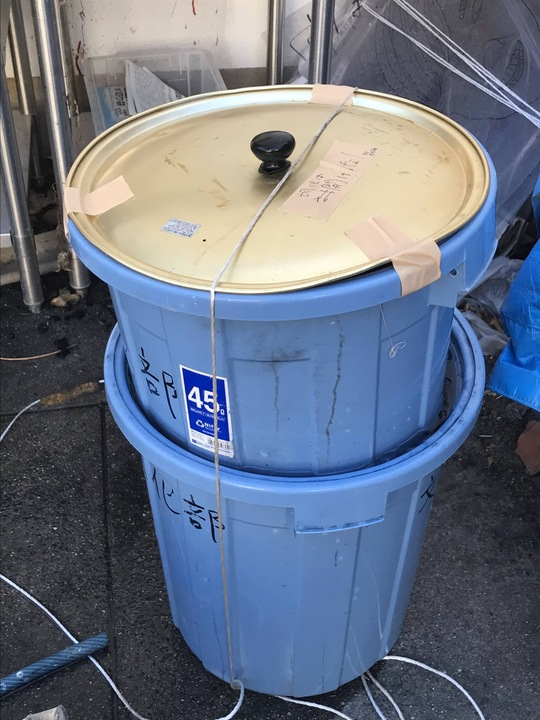
\includegraphics[width=\linewidth,height=3.2cm,keepaspectratio]{2026shinki/kaesaru/images/img_7323_720.jpg}
	\end{minipage}\hfill
	\begin{minipage}[t]{0.32\linewidth}
		\centering
		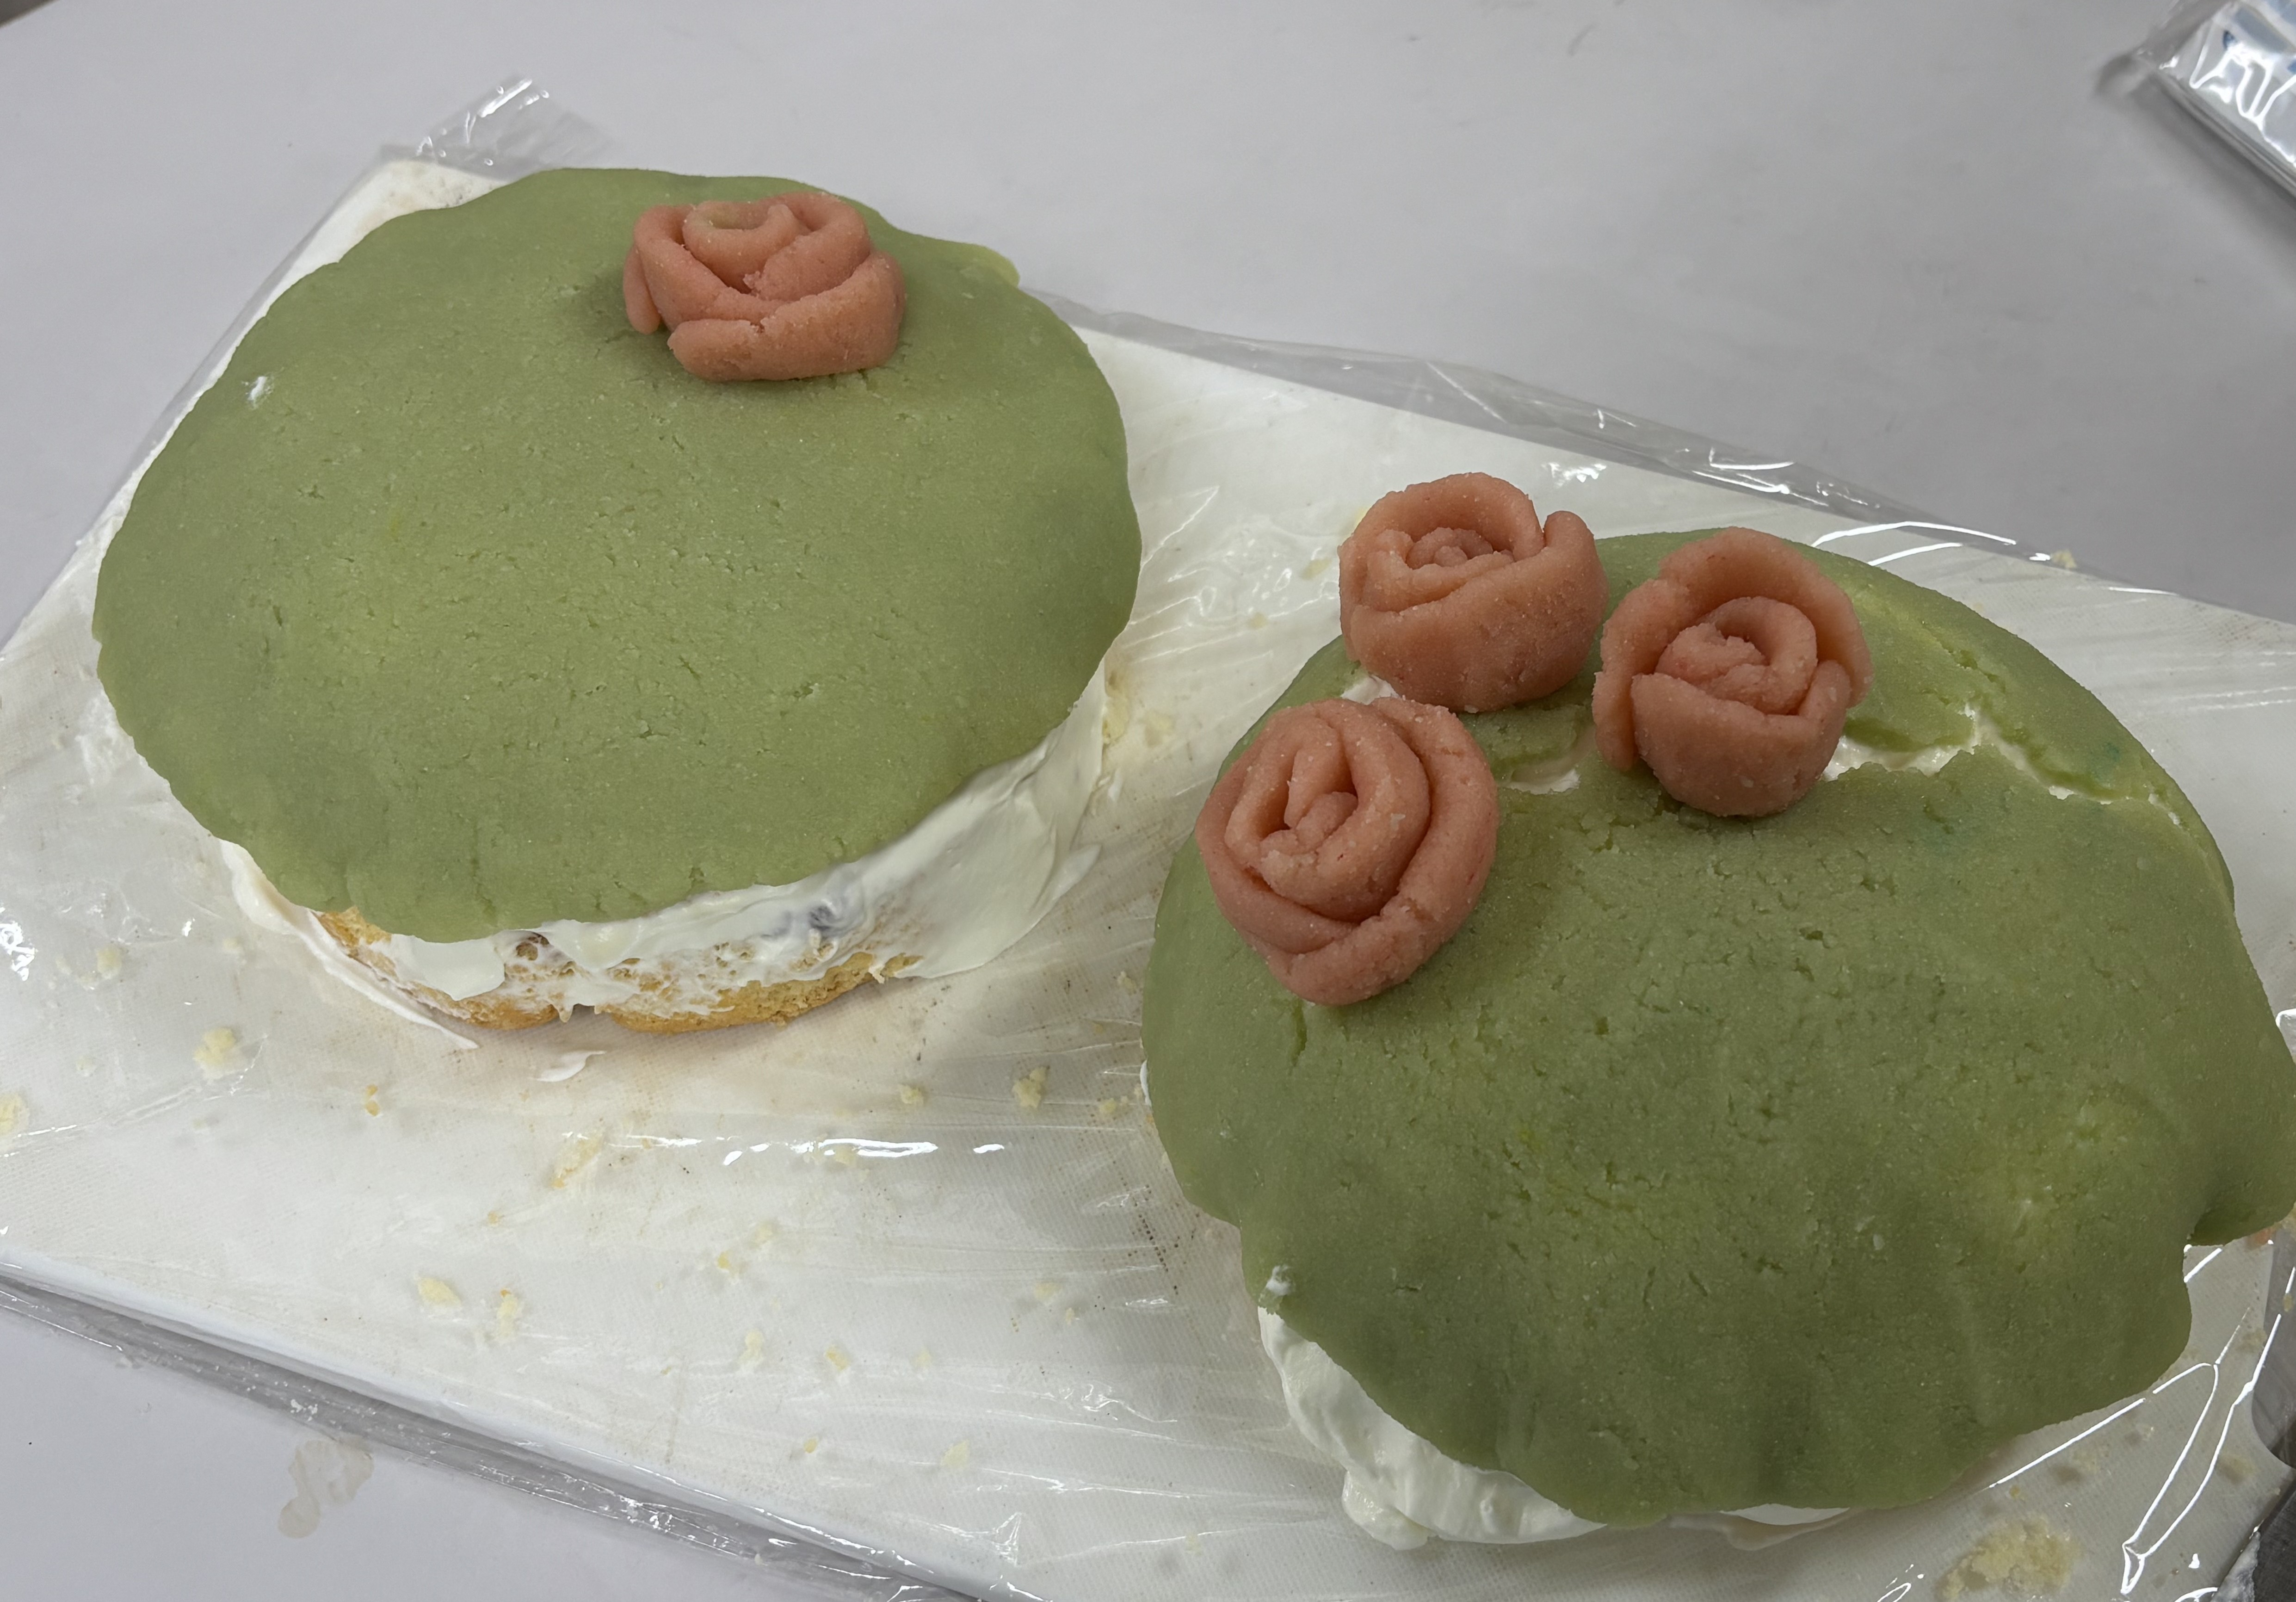
\includegraphics[width=\linewidth,height=3.2cm,keepaspectratio]{2026shinki/kaesaru/images/FF4B2E8A-43ED-4925-B3BE-C4DAB74F0BFF.JPG}
	\end{minipage}\hfill
	\begin{minipage}[t]{0.32\linewidth}
		\centering
		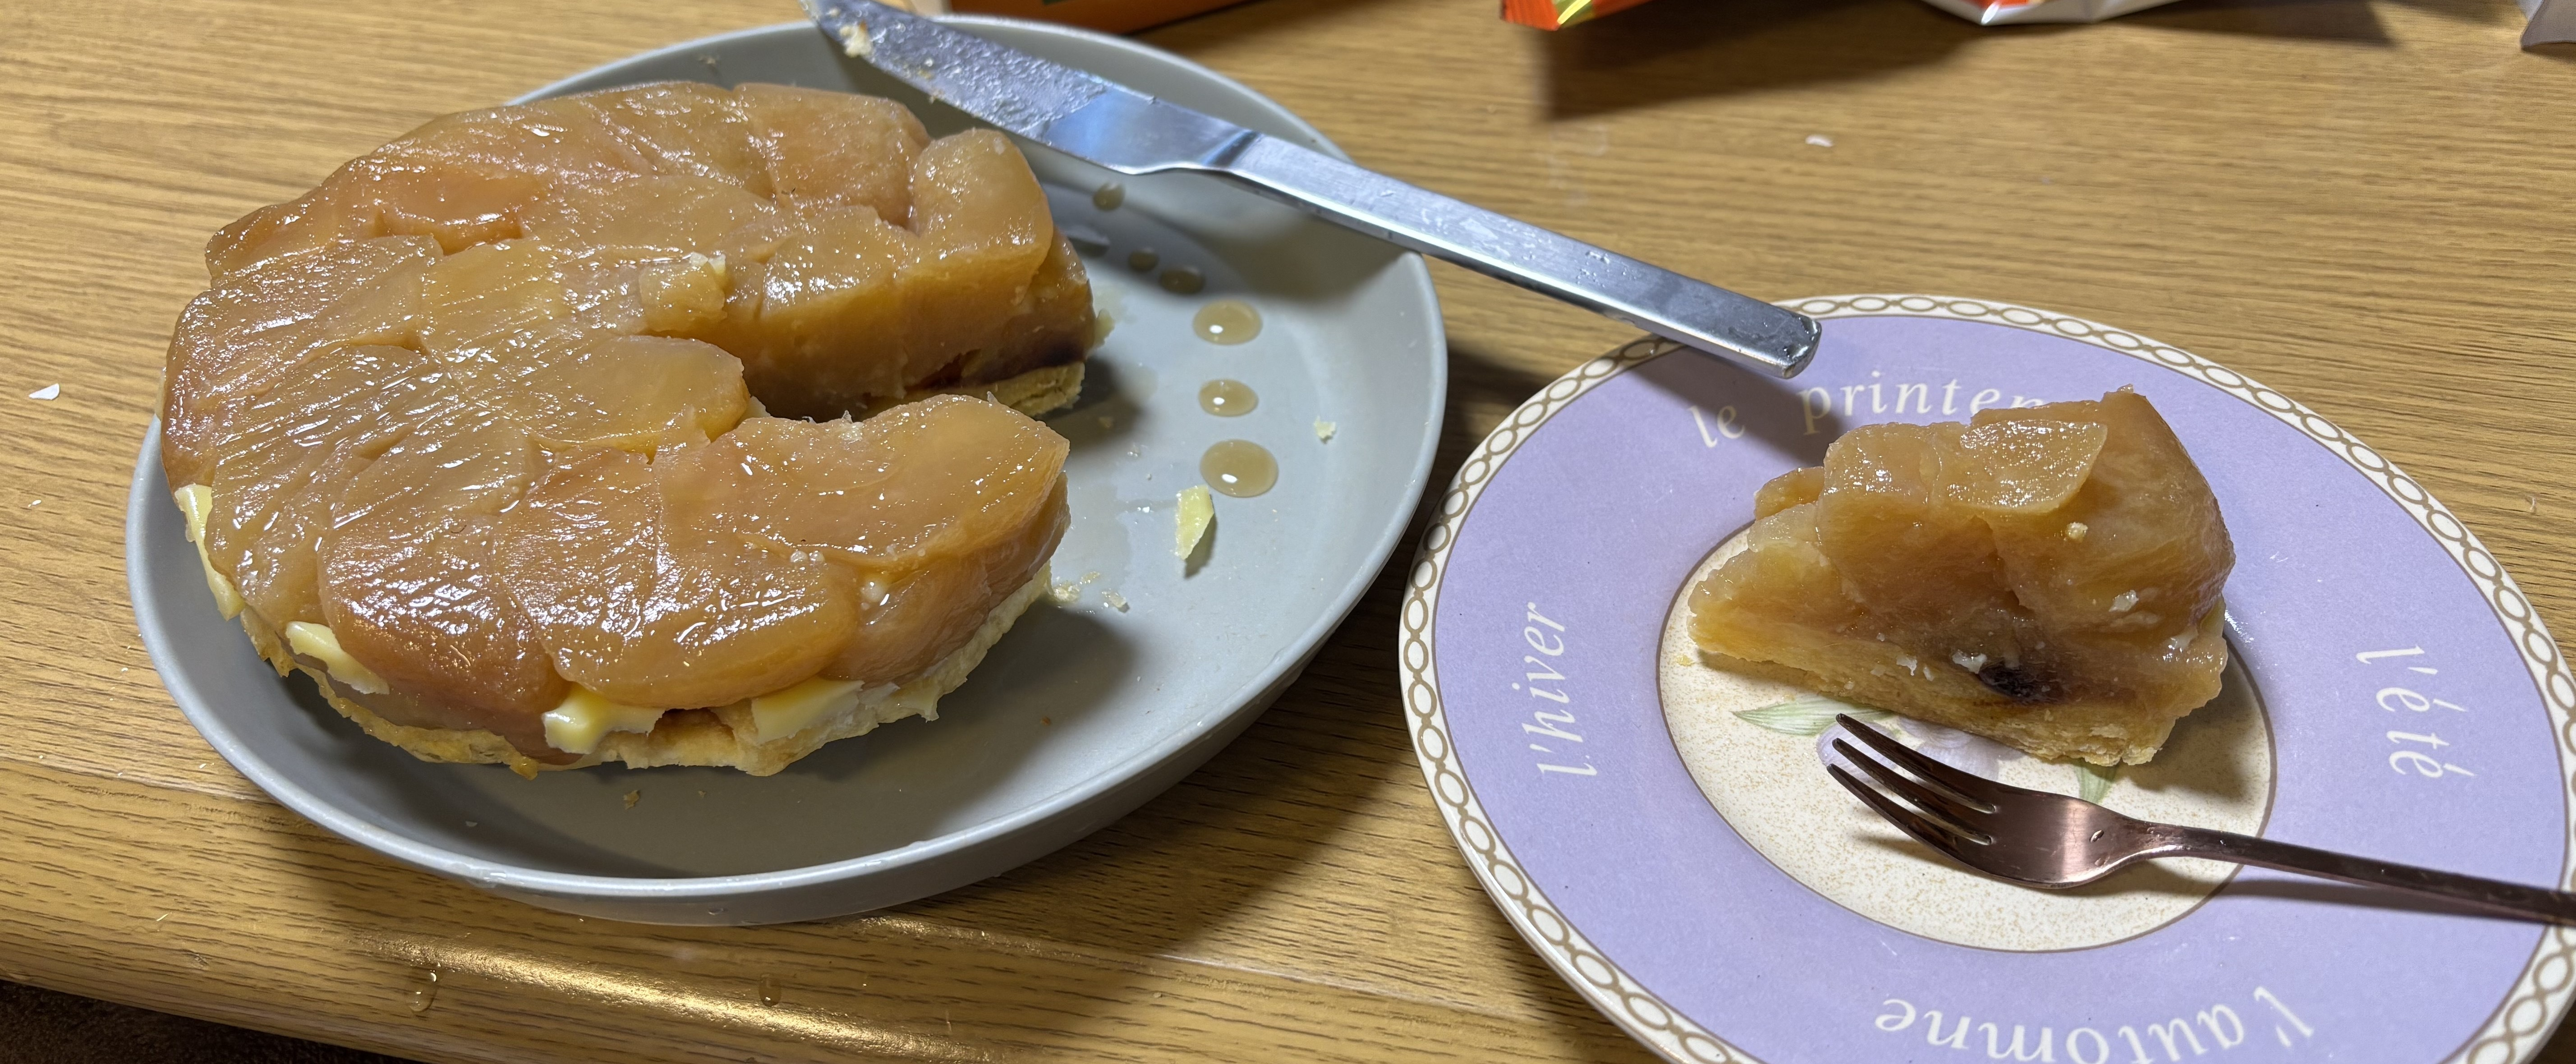
\includegraphics[width=\linewidth,height=3.2cm,keepaspectratio]{2026shinki/kaesaru/images/9886B881-7B81-49BB-825A-F67DB3026609.JPG}
	\end{minipage}
\end{figurehere}

タルト…新入寮生だったがティーパーティー新歓でお菓子を出そうと思った。ところまではよいのだが、なぜか3品以上出すつもりでおり、買い出しや準備の不慣れも相まって当日は大忙しとなった。作るもの自体は実家で作り慣れていたので、それは救いだった。確かクリームチーズタルトだった。
タルトタタン…名前が好き。ケーキ型にりんごを煮たのを入れ、タルト生地の一つをかぶせて焼いた。形を保つのがぎりぎりだったような気がする。
ごま団子…新歓が始まってから作っていた気がする。チョコとあんこ。
ラングドシャ…タルトの卵白消費のレシピ。薄く作らないとおいしくできず、生地を使い切るまでに10回は焼いた気がする。
シュークリーム…卵か牛乳を余らせてしまいカスタードクリームを大量に作った。温度調整がうまくいかず、シュー皮が余り膨らまなかったが味は良かった。辻口シェフの動画のレシピだった気がする。
ぐりとぐらのカステラ…寮祭企画。フライパンのレシピを寮の大きな鍋でやろうとした。体積を等倍にした結果、コンロの下からの火では上部まで加熱できなかった。参加者の機転でクッキングシートを引いたうえでひっくり返したところ、一部のみ焦げるにとどまった。初めての寮祭企画だったが寮外生の参加が多く励みになった。
カラスのパン屋さんのパン…寮祭企画。KUMAN（熊野寮がやっている寺子屋）の子供たちが多く来てくれた。見た目がかわいいパンがたくさんできた。味はシンプルだがおいしかった。
ゴミバケツプリン…寮祭企画。寮のゴミバケツ（の中の飲み物冷やすように使われてるやつ、かなり洗った）を使ってプリンを作った。加熱で固めるのは難しいと思い、寒天で固めるレシピに。鍋で加熱したのをバケツに入れるのを4回くらい繰り返した。取り出すのがドラマチック.味は…。
タルト、プリン…バレンタインコンパ。ティーパーティーより段取りに成長が見られた。このときチョコチップクッキーを、作れる知り合いと未経験者（ゴミバケツプリンを手伝ってもらった寮生）に丸投げしたが、お菓子作りの楽しさを「初めて」知ったと言ってくれた。バケツプリンは味が微妙だったのでね。
キッシュ…同じく。プリンで白身が余ったのを活用。見た目が白いのも面白い。
アイスのタルト…誕生日会.夏だったので。
タルトタタン…おつとめ品のりんごを買ったので作った。グレーテルのかまどのレシピ。力作。
クッキー…鳥獣戯画の型を買ったので。出来立ては格別。
タルト…出町の八百屋でイチゴが一パック250円くらいで売られていた。クリームとも相性◎
バナナのパウンドケーキ…おつとめ品のバナナで作る。一級においしいのに、一級に材料費が安い。私の手札に加わった。
プリンセストルタ…サーターアンダギーコンパで提供。スウェーデンのケーキで緑色のマジパンが被さっている。力作なのだが、なぜ私がスウェーデンのケーキを作ったのか尋ねてほしかった。
シフォンケーキ…新オーブンの初調理。材料のうち卵以外はすべて寮歌ブロックからもらった。塩が少し多かったが、ふわふわ感は素晴らしい。
プリン、バナナのパウンドケーキ…オーブンが大きいと一気に焼けることを実感。

\subsection{おわりに}
　書き出して見ると想像以上の多さにびっくりしました。実家にいた頃は同じもの、同じレシピを作ることが多かったのですが、寮に入ってネットでレシピを調べて、作ったことがないものに挑戦することが増えました。これから寮に入る皆さんにとって熊野寮が住みよい場所であると同時に、挑戦できる環境を提供できる場所であり続けることを目指すとともに願い、結びとさせていただきます。